\documentclass[a4paper,12pt]{article}
%\usepackage{macros}


\usepackage[T1]{fontenc}
\usepackage{lmodern}
\usepackage{amsmath}
\usepackage{amsfonts}
\usepackage{amssymb}
\usepackage{amsthm}
\usepackage{mathrsfs}
\usepackage{physics}
\usepackage{graphicx}
\usepackage{caption}
\usepackage{subcaption}
\usepackage{enumitem}
\usepackage{framed,float}
\usepackage{booktabs}
\usepackage{array}
\usepackage{soul}
\usepackage{multirow}
\usepackage{comment}
\usepackage{braket}
\usepackage{todonotes}
\usepackage{youngtab}
\usepackage{tikz}
\usepackage{slashed}
\usepackage{epstopdf}


\usepackage{geometry}



\renewcommand{\d}{\mathrm{d}}

\begin{document}

\section{RG Flow\cite{Coleman_1985,Deligne:1999qp}}
Broadly speaking, physical theories are scale-dependent. As we move from theories at smaller scales to those at larger scales,
a decouping process occurs, which means information from the smaller scales is effectively packaged and passed on as parameters 
in the theory at the larger scale. Here scale has the dimension of distance. Later it given in energy dimension.\par
In simple terms, renormalization is used to handle the decouping in quantum theories. Quantum theories are described by actions.
Each scale admits many possible theories, and we use correlation function as the basis for determining whether two theories are connected.
An action $S_{eff}$ is called an effective action at the scale $\Lambda_1$ of $S$ at the scale $\Lambda$ if 
the correlation function derived form them are the same.\par
Now we can define a map in the ``theory space'' $R_{\Lambda_1 \Lambda_2}:(S_1,\Lambda_1)\mapsto(S_2,\Lambda_2)$, where
$S_2$ is the effective action at the scale $\Lambda_2$ of $S_1$ at the scale $\Lambda_1$. It is easy to see,
\begin{equation}
    R_{\Lambda_1\Lambda_2}R_{\Lambda_2\Lambda_3}=R_{\Lambda_1\Lambda_3},
\end{equation}    
and
\begin{equation}
    R_{\Lambda \Lambda}=\text{identity map},
\end{equation}
which satisfies the definition of the semi-group. That's the reason for the name, renormalization ``group''. 
If we start from a theory at the scale $\Lambda$ in the space of theories and following this map, we obtain a series
of theories forming something like a flow, which is called the \textbf{RG flow}. In mathematical language,
\begin{equation}
    t(S,\Lambda)=(R_{\Lambda,t \Lambda}S,t \Lambda),\qquad t\in \mathbb{R}^+.
\end{equation}
The decouping process from the action $S$ at the scale $\Lambda$ to its effective Lagrangian $\mathcal{L}_{eff}$ at the scale $\Lambda_1$
 can be described as,
\begin{equation}
    \label{wilson-pic}
e^{-S_{eff}(\phi)}=\int e^{-S(\phi+\eta)}\mathcal{D}\eta.
\end{equation}
The integral is taken over all fields $\eta$ whose Fourier transform is supported in $\Lambda_1 \leq |p|\leq \Lambda$. 


\section{$\beta$ Fuction\cite{Schwartz:2014sze,Peskin:1995ev}}
\subsection{Callan-Symanzik Equation}
In general, equation \eqref{wilson-pic} cannot guarantee the form of Lagrangian $\mathcal{L}$ and $\mathcal{L}_{eff}$ are identical. 
However, we can focus on theories where the Lagrangian structure remains the same, with only the parameters varying with the scales.
In this case, studying how these parameters evolve with scale fully determines how the theory changes under scale changes.
The behavior of there parameters is described by the \textbf{Callan-Symanzik equation},
\begin{equation}
    \bigg[\mu\frac{\partial}{\partial \mu}+\beta(g)\frac{\partial}{\partial g}+n \gamma(g)\bigg]G^{(n)}=0,
\end{equation}
where $G^{(n)}$ is the n-point renormalized Green's function, $\mu$ is the scale, $g$ is the coupling constant and,
\begin{equation}
    \beta \equiv \mu\frac{\d g}{\d \mu}\quad\text{and}\quad \gamma=\frac{Z}{2\mu}\frac{\d Z}{\d \mu},
\end{equation}
where $Z$ is the wave function renormalization factor for the field in this theory. 
For theories with more coupling constants or fields, more terms need to be added.\par
Next, I will compute the one-loop $\beta$-function for QCD.\par
\subsection{QCD}
The Lagrangian for Yang-Mills theory coupling with fermions is
\begin{equation}
    \mathcal{L}=-\frac{1}{2}\tr\big(F^{\mu \nu}F_{\mu \nu}\big)-\frac{1}{2\xi}(\partial\cdot A^a)^2+\tilde{c}^a(-\partial^\mu D_{\mu}^{ac})c^c+\bar{\psi}(i\slashed{D}-m)\psi,
\end{equation}
where
\begin{equation}
    F_{\mu \nu}^a=\partial_\mu A^a_\nu-\partial_\nu A^a_{\mu}+gf^{abc}A_\mu^b A_\nu^c,
\end{equation}
and
\begin{equation}
    D_{\mu}^{ac}=\delta^{ac}\partial_{\mu}+gf^{abc}A^{b}_{\mu}.
\end{equation}
$\xi$ is the gauge parameter, which will be chosen as $1$ in the beta function computation part. After expanding,
\begin{equation}
    \begin{split}
    \mathcal{L}=&-\frac{1}{4}(\partial_{\mu}A_{0\nu}^{a}-\partial_{\nu}A_{0\mu}^{a})^{2}-g_{0}f^{abc}(\partial_{\mu}A_{0\nu}^{a})A_{0}^{\mu b}A_{0}^{\nu c}-\frac{1}{2\xi}(\partial^\mu A^a_{0\mu})^2\\
    &-\frac{1}{4}g_0^{2}(f^{eab}A_{0}^{\mu a}A_{0}^{\nu b})(f^{ecd}A_{0\mu}^{c}A_{0\nu}^{d})-\bar{c}_{0}^{a}\partial^{2}c_{0}^{a}-g_0\bar{c}_{0}^{a}f^{abc}\partial^{\mu}A_{0\mu}^{b}c_{0}^{c}\\
    &+\bar{\psi}_0(i\slashed{\partial}-m_0)\psi_0+g_0 A_{0\mu}^a \bar{\psi}_0 \gamma^\mu t^a \psi_0.
    \end{split}
\end{equation}
The subscript $0$ means they are bare quantities. Changing to renormalized quantities and doing the dimensional regularization ($d=4-\epsilon$),
\begin{equation}
    \begin{split}
    A_0&=Z_3^{1/2}A,\\
    \psi_0&=Z_2^{1/2}\psi,\\
    c_0&=Z_{2c}^{1/2}c,\\
    g_0&=Z_g g \mu^{-\epsilon/2},\\
    m_0&=\frac{m_0}{m}m.
    \end{split}
\end{equation}
\begin{equation}\label{lren}
    \begin{split}
        \mathcal{L}=&-\frac{1}{4}Z_3(\partial_{\mu}A_{\nu}^{a}-\partial_{\nu}A_{\mu}^{a})^{2}-g\mu^{-\epsilon/2} Z_gZ_3^{2/3}f^{abc}(\partial_{\mu}A_{\nu}^{a})A^{\mu b}A^{\nu c}-\frac{1}{2\xi}Z_3(\partial^\mu A^a_{\mu})^2\\
        &-\frac{1}{4}g^{2}\mu^{-\epsilon}Z_g^2 Z_3^2(f^{eab}A^{\mu a}A^{\nu b})(f^{ecd}A_{\mu}^{c}A_{\nu}^{d})-Z_{2c}\bar{c}^{a}\partial^{2}c^{a}-g\mu^{-\epsilon/2} Z_gZ_{2c}(Z_3)^{1/2}\bar{c}^{a}f^{abc}\partial^{\mu}A_{\mu}^{b}c^{c}\\
        &+Z_2\bar{\psi}(i\slashed{\partial}-\frac{m_0}{m} m)\psi+g\mu^{-\epsilon/2} Z_gZ_2(Z_3)^{1/2} A_\mu^a \bar{\psi} \gamma^\mu t^a \psi.
        \end{split}
\end{equation}
This Lagrangian can be splitted to the renormalized part and counter term. renormalized part is simple and I just write down the $\mathcal{L}_{ct}$,
\begin{equation}\label{lct}
    \begin{split}
        \mathcal{L}_{ct}=&-\frac{1}{4}\delta_3(\partial_{\mu}A_{\nu}^{a}-\partial_{\nu}A_{\mu}^{a})^{2}-g\mu^{-\epsilon/2} \delta_{A^3}f^{abc}(\partial_{\mu}A_{\nu}^{a})A^{\mu b}A^{\nu c}-\frac{1}{2\xi}\delta_3(\partial^\mu A^a_{\mu})^2\\
        &-\frac{1}{4}g^{2}\mu^{-\epsilon}\delta_{A^4}(f^{eab}A^{\mu a}A^{\nu b})(f^{ecd}A_{\mu}^{c}A_{\nu}^{d})-\delta_{2c}\bar{c}^{a}\partial^{2}c^{a}-g\mu^{-\epsilon/2} \delta_{1c}\bar{c}^{a}f^{abc}\partial^{\mu}A_{\mu}^{b}c^{c}\\
        &+\bar{\psi}(i \delta_2\slashed{\partial}-\delta_m)\psi + g\mu^{-\epsilon/2} \delta_1 A_\mu^a \bar{\psi} \gamma^\mu t^a \psi.
        \end{split}
\end{equation}
by comparing \eqref{lren} and \eqref{lct}, we can get,
\begin{equation}
    \begin{split}
    \delta_3=Z_3-1,\qquad \delta_{A^3}=Z_3^{2/3}Z_g-1,\qquad \delta_{A^4}=Z_3^2 Z^2_1-1,\\
    \delta_{2c}=Z_{2c}-1,\qquad \delta_{1c}=Z_{2c}(Z_3)^{1/2}Z_g-1,\qquad \delta_2=Z_2-1,\\
    \delta_m=Z_2m_0-m,\qquad \delta_1=Z_2(Z_3)^{1/2}Z_g-1.
    \end{split}
\end{equation}
All these couterterms can be computed by the standard perturbative method (Feynman diagrams). The last equation can be written as,
\begin{equation}
    g_0=g\frac{1+\delta_1}{Z_2(Z_3)^{1/2}}\mu^{\epsilon/2}.
\end{equation}
Now we can get a simple formula for $\beta$ function from the scale independence of bare quantities ($\frac{\d g_0}{\d\mu}=0$),
\begin{equation}
    \begin{split}
    \beta(g)=&\mu\frac{\d}{\d \mu}g=g\bigg[\Big(-\frac{\epsilon}{2}\Big)-\mu\frac{\d}{\d \mu}\bigg(\delta_1-\delta_2-\frac{1}{2}\delta_3\bigg)\bigg]+\cdots\\
        =&g\bigg[\Big(-\frac{\epsilon}{2}\Big)-\mu\frac{\d g}{\d \mu}\frac{\partial}{\partial g}\bigg(\delta_1-\delta_2-\frac{1}{2}\delta_3\bigg)\bigg]+\cdots\\
        =&g\bigg[\Big(-\frac{\epsilon}{2}\Big)-\beta(g)\frac{\partial}{\partial g}\bigg(\delta_1-\delta_2-\frac{1}{2}\delta_3\bigg)\bigg]+\cdots
\end{split}
\end{equation}
At one-loop, $\delta\propto g^2$. So if I only compute $\beta(g)$ up to $g^3$, the $\beta(g)$ in the right hand side can be taken as $-\frac{\epsilon}{2}g$, 
and the higher-order terms are thrown into the dots, i.e.
\begin{equation}\label{beta}
    \beta(g)=-\frac{\epsilon}{2}g+\frac{\epsilon}{2}g^2\frac{\partial}{\partial g}\bigg(\delta_1-\delta_2-\frac{1}{2}\delta_3\bigg)+\cdots
\end{equation}

\subsection{One-Loop $\beta$ Function For QCD}
Now I begin to compute the three couterterms $\delta_1,\delta_2$ and $\delta_3$.\par
$\delta_3$ is the counterterm for the gluon self-energy. At one-loop,

\begin{center}
    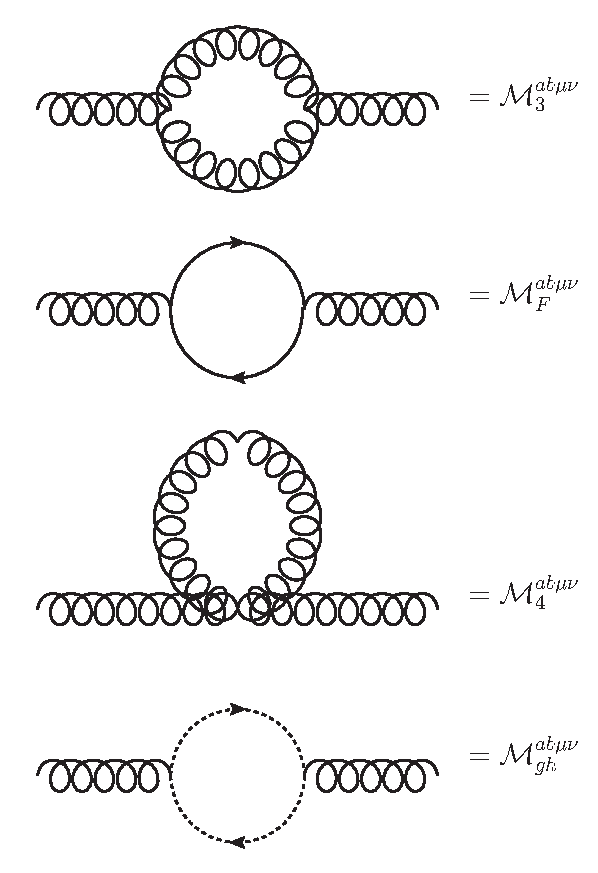
\includegraphics{rgf/gluonse.eps}
\end{center}
and our counterterm $\delta_3$. Since Feynman rules are not the focus here, I will omit them. Nevertheless, we can use them to get the expressions for these diagrams.
\begin{equation}
    \begin{split}
        &i\mathcal{M}_{F}^{ab \mu \nu}\\
        =&-\tr[T^{a}T^{b}](ig)^{2}\int\frac{\d^{4}k}{(2\pi)^{4}}\frac{i}{(p-k)^{2}-m^{2}}\frac{i}{k^{2}-m^{2}}\tr[\gamma^{\mu}(\slashed k-\slashed p+m)\gamma^{\nu}(\slashed k+m)]\\
        =&-\frac{1}{2}\delta^{ab}g^2\int\frac{\d^{4}k}{(2\pi)^{4}}\frac{4[-p^{\mu}k^{\nu}-k^{\mu}p^{\nu}+2k^{\mu}k^{\nu}+g^{\mu\nu}(-k^{2}+p\cdot k+m^{2})]}{[(p-k)^{2}-m^{2}+i \epsilon][k^{2}-m^{2}+i \epsilon]}
    \end{split}
\end{equation}
We know Feynman parameters,
\begin{equation}
    \frac{1}{AB}=\int_0^1 \d x\frac{1}{[xA+(1-x)B]^2}.
\end{equation}
By using this,
\begin{equation}
    \mathcal{M}_{F}^{ab \mu \nu}
        =2i\delta^{ab}g^2\int\frac{\d^{4}k}{(2\pi)^{4}}\int_0^1 \d x \frac{-p^{\mu}k^{\nu}-k^{\mu}p^{\nu}+2k^{\mu}k^{\nu}+g^{\mu\nu}(-k^{2}+p\cdot k+m^{2})}{[k^2+p^2x-2k\cdot p x-m^2+i \epsilon]^2}.
\end{equation}
We do not want to see the $k\cdot p$ term in the denominator, so we use $k^{'\mu}=k^\mu-xp^\mu$  to replace $k$. 
Since this is a full integration over momentum, this transformation will not affect the overall result of the integral.
\begin{equation}
    \mathcal{M}_{F}^{ab \mu \nu}
        =2i\delta^{ab}g^2\int\frac{\d^{4}k}{(2\pi)^{4}}\int_0^1 \d x \frac{2k^{\mu}k^{\nu}-g^{\mu\nu}[k^{2}-p^2x(1-x)-m^{2}]+2x(x-1)p^\mu p^\nu}{[k^2+p^2x(1-x)-m^2+i \epsilon]^2}.
\end{equation}
Here $k$ means $k'$. I omit the $pk'$-form terms since they are the odd function of $k$ and vanishing after integral. 
By using dimensional regularization and $k^\mu k^\nu=\frac{1}{d}g^{\mu \nu}k^2$ in $d$ dimensions,  
\begin{equation}
    \mathcal{M}_{F}^{ab \mu \nu}
        =2i\delta^{ab}g^2\mu^{4-d}\int\frac{\d^{d}k}{(2\pi)^{d}}\int_0^1 \d x \frac{-g^{\mu\nu}[(1-\frac{2}{d})k^{2}-p^2x(1-x)-m^{2}]+2x(x-1)p^\mu p^\nu}{[k^2+p^2x(1-x)-m^2+i \epsilon]^2}.
\end{equation}
We have formula for this kind of integral,
\begin{equation}
    \int\frac{\d^d k}{(2\pi)^d}\frac{k^2}{(k^2-\Delta+i \epsilon)^2}=-\frac{d}{2}\frac{i}{(4\pi)^{\frac{d}{2}}}\frac{1}{\Delta^{1-\frac{d}{2}}}\Gamma\Big(\frac{2-d}{2}\Big)
\end{equation}
\begin{equation}
    \int\frac{\d^d k}{(2\pi)^d}\frac{k^2}{(k^2-\Delta+i \epsilon)^2}=\frac{i}{(4\pi)^{\frac{d}{2}}}\frac{1}{\Delta^{2-\frac{d}{2}}}\Gamma\Big(\frac{4-d}{2}\Big)
\end{equation}
Now we have,
\begin{equation}
    \begin{split}
    \mathcal{M}_{F}^{ab \mu \nu}&=2i \delta^{ab}g^2 \mu^{4-d}\times\\
    &\Bigg\{-g^{\mu \nu}\Big(1-\frac{d}{2}\Big)\Gamma\Big(1-\frac{d}{2}\Big)\frac{i}{(4\pi)^{\frac{d}{2}}}\int_0^1 \d x\frac{1}{\Delta^{1-\frac{d}{2}}}+g^{\mu \nu}\Gamma\Big(2-\frac{d}{2}\Big)\frac{i}{(4\pi)^{\frac{d}{2}}}\int_0^1 \d x\frac{p^2x(1-x)}{\Delta^{2-\frac{d}{2}}}\\
    &+g^{\mu \nu}\Gamma\Big(2-\frac{d}{2}\Big)\frac{i}{(4\pi)^{\frac{d}{2}}}\int_0^1 \d x\frac{m^2}{\Delta^{2-\frac{d}{2}}}+p^\mu p^\nu\Gamma\Big(2-\frac{d}{2}\Big)\frac{i}{(4\pi)^{\frac{d}{2}}}\int_0^1 \d x\frac{x(x-1)}{\Delta^{2-\frac{d}{2}}}\Bigg\}\\
    =&-2\delta^{ab}g^2 \mu^{4-d}\Gamma\Big(2-\frac{d}{2}\Big)\frac{1}{(4\pi)^{\frac{d}{2}}}\times\\
    &\Bigg\{g^{\mu \nu}\int_0^1 \d x\frac{-\Delta+p^2x(1-x)+m^2}{\Delta^{2-\frac{d}{2}}}+p^\mu p^\nu\int_0^1 \d x\frac{x(x-1)}{\Delta^{2-\frac{d}{2}}}\Bigg\}\\
    =&-2\delta^{ab}g^2 \mu^{4-d}\Gamma\Big(2-\frac{d}{2}\Big)\frac{1}{(4\pi)^{\frac{d}{2}}}(p^2g^{\mu \nu}-p^\mu p^\nu)\times\int_0^1 \d x\frac{2x(1-x)}{(m^2-p^2x(1-x))^{2-\frac{d}{2}}}\\
    =&\frac{-\delta^{ab}g^2}{8\pi^2} \Gamma\Big(\frac{\epsilon}{2}\Big)(p^2g^{\mu \nu}-p^\mu p^\nu)\times\int_0^1 \d x\,2x(1-x)\bigg(\frac{4\pi \mu^2}{m^2-p^2x(1-x)}\bigg)^{\frac{\epsilon}{2}}
\end{split}
\end{equation}
with $\Delta=m^2-p^2x(1-x)$ and $\epsilon=4-d$. In the limit $\epsilon\to 0$,

\begin{equation}
    \begin{split}
    &\mathcal{M}_{F}^{ab \mu \nu}\\
    =&\frac{-\delta^{ab}g^2}{8\pi^2} (p^2g^{\mu \nu}-p^\mu p^\nu)\Big(\frac{2}{\epsilon}-\gamma_E+\mathcal{O}(\epsilon)\Big)\int_0^1 \d x\,2x(1-x)\bigg[1+\frac{\epsilon}{2}\ln\bigg(\frac{4\pi \mu^2}{m^2-p^2x(1-x)}\bigg)+\mathcal{O}(\epsilon^2) \bigg]\\
    =&\frac{-\delta^{ab}g^2}{8\pi^2} (p^2g^{\mu \nu}-p^\mu p^\nu)\int_0^1 \d x\,2x(1-x)\bigg[\frac{2}{\epsilon}+\ln\bigg(\frac{4\pi e^{-\gamma_E}\mu^2}{m^2-p^2x(1-x)}\bigg)+\mathcal{O}(\epsilon) \bigg]\\
    =&\frac{\delta^{ab}g^2}{(4\pi)^2} (p^2g^{\mu \nu}-p^\mu p^\nu)\bigg[-\frac{4}{3}\frac{1}{\epsilon}+(finite) \bigg],
    \end{split}
\end{equation}
where $x^{\epsilon/2}=1+\frac{\epsilon}{2}\ln x+\cdots$ and $\Gamma(\epsilon/2)=\frac{2}{\epsilon}-\gamma_E+\cdots$ are used. If we have $n_f$ species of fermions in the same representation, the total contribution will be,
\begin{equation}
    \frac{\delta^{ab}g^2}{(4\pi^2)^2} (p^2g^{\mu \nu}-p^\mu p^\nu)\bigg[-\frac{4}{3}n_f\frac{1}{\epsilon}+(finite) \bigg].
\end{equation}
Now the contribution from the gluon bubble,
\begin{equation}
    i\mathcal{M}_3^{ab \mu \nu}=\frac{g^2}{2}\int \frac{\d^4 k}{(2\pi)^4}\int \frac{\d^4 k}{(2\pi)^4}\frac{-i}{k^2}\frac{-i}{(k-p)^2}f^{acd}f^{bdc}N^{\mu \nu}.
\end{equation}
The numerator is,
\begin{equation}
    \begin{split}
        N^{\mu\nu}=&\left[g^{\mu\alpha}\left(p+k\right)^{\rho}+g^{\alpha\rho}\left(p-2k\right)^{\mu}+g^{\rho\mu}\left(k-2p\right)^{\alpha}\right]g_{\alpha\beta}g_{\rho\sigma}\\
        &\times\left[g^{\nu\beta}(p+k)^{\sigma}-g^{\beta\sigma}(2k-p)^{\nu}-g^{\sigma\nu}(2p-k)^{\beta}\right].
    \end{split}
\end{equation}
Also introducing Feynman parameters with $\Delta=x(x-1)p^2$  and using dimensional regularization, we can get,
\begin{equation}
    \begin{split}
        \mathcal{M}_{3}^{ab\mu\nu}=&-\frac{g^{2}}{2}\frac{\mu^{4-d}}{\left(4\pi\right)^{d/2}}\delta^{ab}C_{A}\int_{0}^{1}\d x\biggl(\frac{1}{\Delta}\biggr)^{2-\frac{d}{2}}\times\bigg\{g^{\mu\nu}3(d-1) \Gamma\biggl(1-\frac{d}{2}\biggr)\Delta\\
        &+p^{\mu}p^{\nu}\bigg[6\big(x^{2}-x+1\big)-d\big(1-2x\big)^{2}\bigg]\Gamma\bigg(2-\frac{d}{2}\bigg)\\
        &+ g^{\mu\nu}p^{2}\bigg[\left(-2x^{2}+2x-5\right)\Gamma\bigg(2-\frac{d}{2}\bigg)\bigg]\bigg\}
    \end{split}
\end{equation}
where $C_A$ is defined by $f^{acd}f^{bcd}=C_A\delta^{ab}$.\par
Then the contribution from the four-point vertex, given by Feynman rule,
\begin{equation}
    \begin{split}
        i\mathcal{M}_{4}^{ab\mu\nu}=
        &-\frac{ig^{2}}{2}\mu^{4-d}\int\frac{\d^{d}k}{\left(2\pi\right)^{d}}\frac{-ig_{\rho\sigma}}{k^{2}+i\varepsilon}\\
        &\times[f^{abe}f^{cde}\delta^{cd}(g^{\mu\rho}g^{\nu\sigma}-g^{\mu\sigma}g^{\nu\rho})+f^{ace}f^{bce}(g^{\mu\nu}g^{\rho\sigma}-g^{\mu\sigma}g^{\nu\rho})\\
        &+f^{ace}f^{bce}(g^{\mu\nu}g^{\rho\sigma}-g^{\mu\rho}g^{\nu\sigma})\Big]\\
        =&-g^{2}\delta^{ab}g^{\mu\nu}C_{A}(d-1)\mu^{4-d}\int\frac{\d^{d}k}{\left(2\pi\right)^{d}}\frac{1}{k^{2}+i\varepsilon}=0,
    \end{split}
\end{equation}
Even though this integral is vanishing, I write it in the Feynman parameter for further computation,
\begin{equation}
    \begin{split}
        \mathcal{M}_4^{ab\mu\nu}=&-g^{2}\delta^{ab}C_{A}\frac{\mu^{4-d}}{\left(4\pi\right)^{d/2}}g^{\mu\nu}\int_{0}^{1}\d x\left(\frac{1}{\Delta}\right)^{2-\frac{d}{2}}(d-1)\\
        &\times\left[-\frac{d}{2}\Gamma\left(1-\frac{d}{2}\right)\Delta+\left(1-x\right)^{2}p^{2}\Gamma\left(2-\frac{d}{2}\right)\right],
    \end{split}
\end{equation}
where $\Delta=x(x-1)p^2$ as well.\par
The final contribution to the gluon self-energy is the ghost bubble,
\begin{equation}
    i \mathcal{M}_{gh}^{ab \mu \nu}=-g^2\int\frac{\d^4k}{(2\pi)^4}\frac{i}{(k-p)^2}\frac{i}{k^2}f^{cad}k^\mu f^{dbc}(k-p)^\nu,
\end{equation}
again,
\begin{equation}
    \begin{split}
        \mathcal{M}_{\mathrm{gh}}^{ab\mu\nu}=&g^{2}\frac{\mu^{4-d}}{\left(4\pi\right)^{d/2}}\delta^{ab}C_{A}\int_{0}^{1}\d x\biggl(\frac{1}{\Delta}\biggr)^{2-\frac{d}{2}}\left\{g^{\mu\nu}\biggl[\frac{1}{2}\Gamma\biggl(1-\frac{d}{2}\biggr)\Delta\biggr]\right.\\
        &+p^{\mu}p^{\nu}\bigg[x(1-x)\Gamma\bigg(2-\frac{d}{2}\bigg)\bigg]\bigg\}.
    \end{split}
\end{equation}
Also using the $\epsilon=4-d$ and in the $\epsilon\to 0$ limit,
\begin{equation}
    \mathcal{M}_{3}^{ab \mu \nu}+\mathcal{M}_{4}^{ab \mu \nu}+\mathcal{M}_{gh}^{ab \mu \nu}=\frac{\delta^{ab}g^2}{(4\pi)^2}(p^2g^{\mu \nu}-p^\mu p^\nu)\bigg[\frac{10}{3}C_A\frac{1}{\epsilon}+(finite)\bigg].
\end{equation}  
The full gluon self energy with counterterm is,
\begin{equation}
    \mathcal{M}^{ab \mu \nu}=\delta^{ab}(p^2g^{\mu \nu}-p^\mu p^\nu)\bigg[\frac{g^2}{16\pi^2}\bigg(\frac{10}{3}C_A-\frac{4}{3}n_f\bigg)\frac{1}{\epsilon}-\delta_3\bigg]+(finite)
\end{equation}
Now we can get the value of counterterm $\delta_3$,
\begin{equation}
    \delta_3=\frac{1}{\epsilon}\frac{g^2}{16\pi^2}\bigg(\frac{10}{3}C_A-\frac{4}{3}n_f\bigg).
\end{equation}
The one-loop quark self-energy diagram is
\begin{center}
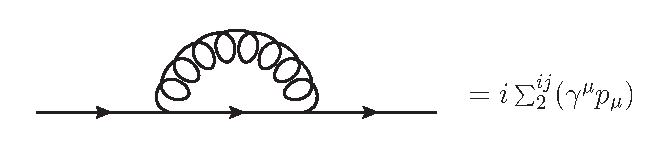
\includegraphics{rgf/fse.eps}
\end{center}
The Feynman rule gives,
\begin{equation}
    i{\Sigma}_2^{ij}(\slashed p)=(t^a)^{il}(t^a)^{lj}(ig)^2\int\frac{\d^4k}{(2\pi)^4}\gamma^\mu \frac{i(\slashed k+m)}{k^2-m^2+i \epsilon}\gamma_\mu\frac{-i}{(k-p)^2+i \epsilon}.
\end{equation}
Adding counterterms $\delta_2$, $\delta_m$ and computing this integral,
\begin{equation}
    {\Sigma}_2^{ij}(\slashed p)=\delta^{ij}\left\{\frac{g^2}{16\pi^2}C_F\left(\frac{2\slashed{p}-8m}{\varepsilon}\right)+\delta_2\slashed p-(\delta_m+\delta_2)m\right\}+(finite),
\end{equation}  
where $C_F$ is defined by $(t^a)_{il}(t^a)_{lj}=C_F \delta_{ij}$, which is $C_F=\frac{N^2-1}{2N}$ for $SU(N)$-gauge theory. Now we can get the counterterm $\delta_2$,
\begin{equation}
    \delta_2=\frac{1}{\epsilon}\frac{g^2}{16\pi^2}(-2C_F).
\end{equation} 
Finally, the counterterm $\delta_1$ is for the gluon-fermion interaction, which has two diagrams in one-loop level,
\begin{center}
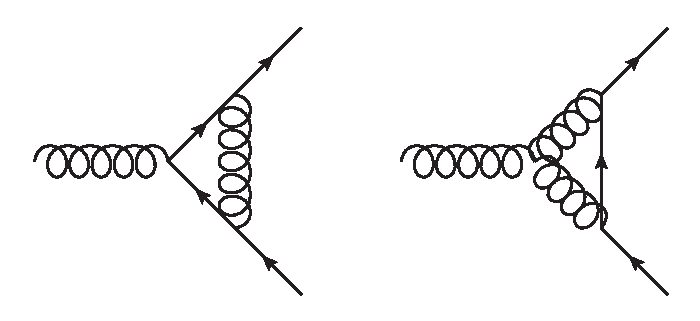
\includegraphics{rgf/3p.eps}
\end{center}
After computation, the counterterm $\delta_1$ is,
\begin{equation}
    \delta_1=\frac{1}{\epsilon}\frac{g^2}{16\pi^2}(-2C_F-2C_A).
\end{equation}
After getting all counterterms we need in equation \eqref{beta}, the beta-function at one-loop is,
\begin{equation}
    \begin{split}
        \beta(g)=&-\frac{\epsilon}{2}g+\frac{1}{2}g^2\frac{\partial}{\partial g}\bigg[\bigg(-\frac{11}{3}C_A+\frac{2}{3}n_f\bigg)\frac{g^2}{16 \pi^2}\bigg]\\
            =&-\frac{\epsilon}{2}g-\frac{g^3}{16 \pi}\bigg[\frac{11}{3}C_A-\frac{2}{3}n_f\bigg].
    \end{split}
\end{equation}
The Casimir of the adjoint representation $C_A=N$ for $SU(N)$-gauge theory. In QCD case, $N=3$ and the flavour number $n_f=6$,
\begin{equation}
    \beta_{\text{QCD}}(g)=-\frac{\epsilon}{2}g-\frac{7g^3}{16\pi^2}<0 
\end{equation}
According to the definition of the beta function, when it is negative, it indicates that the coupling constant decreases at high energy. This is known as asymptotic freedom.
\bibliographystyle{unsrt}
\bibliography{rg}
\end{document}